\documentclass{beamer}
%\usecolortheme{seahorse} % change this
\usepackage{graphicx}
\usepackage{inconsolata}
\usepackage{anyfontsize}
\usepackage{courier}



\usepackage{natbib} 
%bibstyle muss einer da sein, 
% setimmt wie der kram an \cite aussieht.
% https://de.wikibooks.org/wiki/LaTeX-W%C3%B6rterbuch:_bibliographystyle
%https://de.sharelatex.com/learn/Bibtex_bibliography_styles
%\bibliographystyle{abbrvnat} 
%\bibliographystyle{unsrt} 
\bibliographystyle{plainnat}




\title 
{A constructive approach for graph concepts
with long range dependencies}
\author % NEEDS MOAR INFO ,, contact etc
%{Stefan Mautner }
{\underline{Stefan Mautner} \and Fabrizio Costa
    \small{ 
        \texttt{
            \href{mailto:mautner@informatik.uni-freiburg.de}
            {mautner@informatik.uni-freiburg.de}}
        \texttt{
            \href{mailto:costa@informatik.uni-freiburg.de}
            {costa@informatik.uni-freiburg.de}}}
}

\date 
{Freiburg University, Chair of Bioinformatics, 2016-12-09}

\titlegraphic{
\includegraphics[width=2cm]{images/logo.jpg}
}

\begin{document}
\frame{\titlepage}



% design goals
\begin{frame}
\frametitle{Design goals for graph construction}

    ~\\
    \emph{The constructive learning problem for finite samples}\footnote{\cite{costa16}}
    ~\\
    ~\\
    \begin{itemize}
        \item optimize for two goals:
            \begin{enumerate}
        \item similar probability density to train set (compare trained estimators)
        \item generated instances should  differ from originals
            \end{enumerate}
    \end{itemize}
    ~\\
    ~\\
    \Large{${argmin}_{\theta}~~L(f_{G_0}(G),f_{G_{\theta}}(G))+
    \lambda{{K(G_0,G_{\theta})}\over{\sqrt{K(G_0,G_0),K(G_{\theta},G_{\theta})}}} $}
\end{frame}


% so far we have the basic graphlearn
\begin{frame}
    \frametitle{Basic algorithm}
    Metropolis--Hastings Algorithm (Markov Chain Simulation)
    \begin{enumerate}
        \item start with training graph
        \item alter graph
        \item decide whether or not to accept proposed change $\rightarrow$ goto 2
    \end{enumerate}
    \pause
    Graph Grammar to increase quality of proposals
    \begin{itemize}
        \item extract graph fragments (neighborhood graphs we call
            CIPs) from training set;
            use them to alter graph as follows:
    \end{itemize}
    %IMAGE OF SOMETHING  

    \begin{columns}
        \column{0.6\textwidth}
    \begin{figure}[ht]
        \centering
        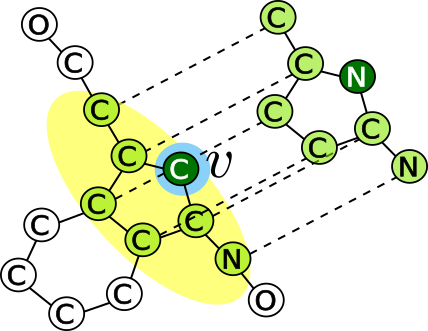
\includegraphics[width=0.66\textwidth]{images/CIP_replacement.png}
    \end{figure}
    \column{.4\textwidth}
        CIP: Core-Interface Pair\\
        yellow: interface\\
        blue: core
    \end{columns}
    
    \small{A replacement can take place if CIPs are \emph{congruent}  }
\end{frame}





% problem with RNA 
\begin{frame}
    \frametitle{The Problem (explained on an RNA structure graph)}
    When graphs become larger..
    \begin{itemize}
        \item want to operate on a higher level 
        \item current grammars local constraints might not be enough
    \end{itemize}
   \begin{figure}[h!]
        \centering
        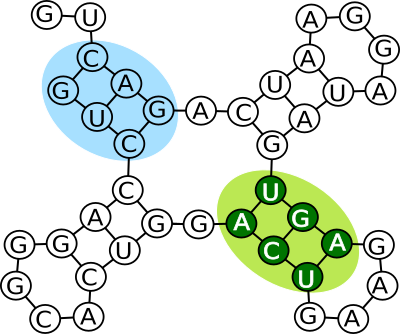
\includegraphics[width=0.33\textwidth]{images/longrangedep.png}
    \end{figure}
    
    \begin{itemize}
        \item (green) use whole ``stem'' as basis for operations
        \item (blue+green) example for a long range dependency; the spheres
            might depend on the presence of one another
    \end{itemize}
\end{frame}



% solution
\begin{frame}
    \frametitle{The Solution}
   \begin{figure}[ht]
        \centering
        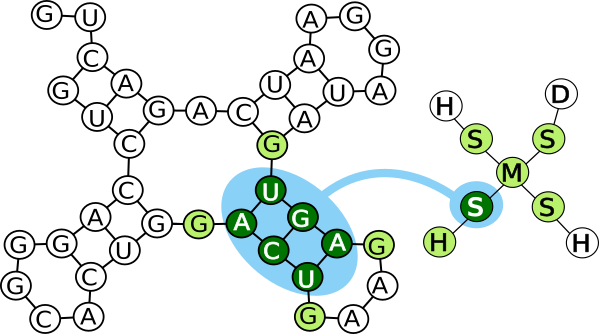
\includegraphics[width=0.50\textwidth]{images/nucip.png}
    \end{figure}
    \begin{itemize}
        \item find a way to abstract your graph (right)
        \item redefine core as nodes from the base graph, induced by the 
            abstract graph (dark green)
        \item redefine Interface-graph as nodes around the core,
            congruency check for CIPs includes the abstract interface
   \end{itemize}
   CIPs have a flexible shape now and include information about their surroundings
   from the abstract graph
\end{frame}





% BENCHMARK I 
\begin{frame}
    \frametitle{Evaluation I}
    \begin{itemize}
        \item we used this method to generate RNA sequences
        \item rfam/Infernal offers a domain specific  way to evaluate sequences
        \item also trained an Infernal model under similar conditions 
            and compared their performance
    \end{itemize}

   \begin{figure}[ht]
        \centering
        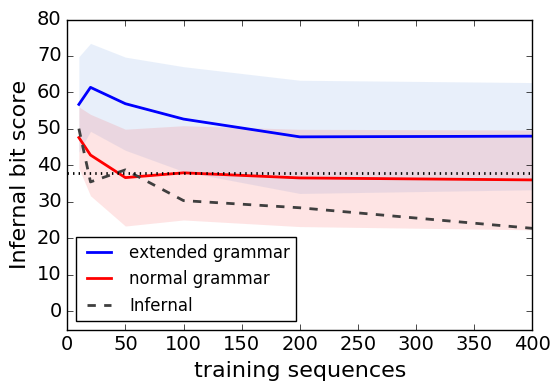
\includegraphics[width=0.60\textwidth]{images/infernal_abstr.png}
    \end{figure}
   \small{horizontal:  the human determined reliability threshold for this RNA family}
\end{frame}

% BENCHMARK II
\begin{frame}
    \frametitle{Evaluation II}
    
    \begin{itemize}
        \item similarity of the generated set vs the train set
        \item Kullback Leibler divergence to measure the difference in probability distribution
    \end{itemize}
   \begin{figure}[ht]
        \centering
        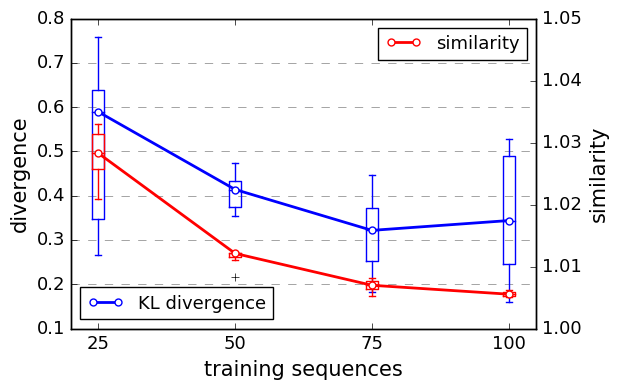
\includegraphics[width=0.6\textwidth]{images/learningcurve.png}
    \end{figure}
     design goal: {${argmin}_{\theta}~~L(f_{G_0}(G),f_{G_{\theta}}(G))+
    \lambda{{K(G_0,G_{\theta})}\over{\sqrt{K(G_0,G_0),K(G_{\theta},G_{\theta})}}} $}

    \tiny{KL Divergence:  $D_{\mathrm{KL}}(P\|Q) = \sum_i P(i) \, \log\frac{P(i)}{Q(i)}$ }
    % IMAGE OF other thing
\end{frame}

% OWARI DA 
\begin{frame}
    \frametitle{Conclusion}
    %\begin{itemize}
        Use the information of abstractions
        to increase the power of your graph grammar!
    %\end{itemize}
\end{frame}
% OWARI DA 
\begin{frame}
    \frametitle{Further Reading}
\bibliography{mybib}
\end{frame}


\end{document}
